\documentclass[tikz,border=4pt]{standalone}
\begin{document}
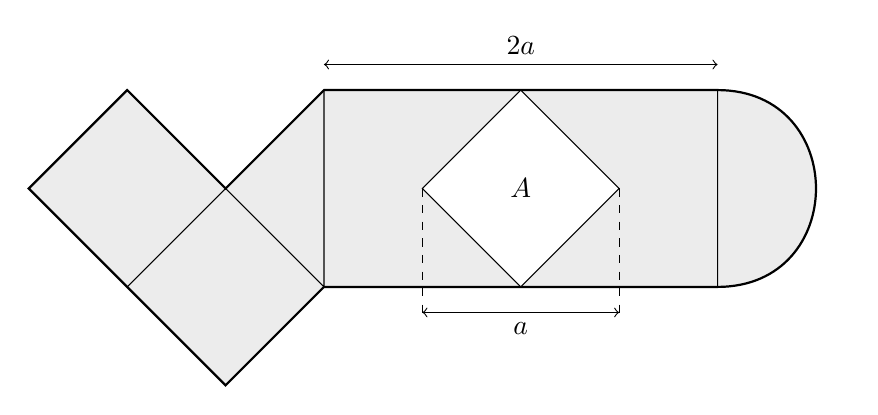
\begin{tikzpicture}[x=0.025cm,y=-0.025cm]
\path[fill=gray!15,draw=black,thick] (20,100)--(70,50)--(120,100)--(170,50)--(370,50) .. controls (436.667,50) and (436.667,150) .. (370,150) -- (170,150)--(120,200)--cycle;
\draw (70,150)--(120,100)--(170,150) (170,50)--(170,150) (370,50)--(370,150);
\path[fill=white,draw=black] (220,100)--(270,50)--(320,100)--(270,150)--cycle;
\draw[<->] (170,37)--node[above]{$2a$}(370,37);
\draw[dashed] (220,100)--(220,167) (320,100)--(320,167);
\draw[<->] (220,163)--node[below]{$a$}(320,163);
\node at (270,100) {$A$};
\end{tikzpicture}
\end{document}
